% Template for PLoS
% Version 1.0 January 2009
%
% To compile to pdf, run:
% latex plos.template
% bibtex plos.template
% latex plos.template
% latex plos.template
% dvipdf plos.template

\documentclass[10pt]{article}

\usepackage{graphicx}
\usepackage{latexsym}
\usepackage{amsfonts,amsmath,amssymb}
\usepackage{url}
\usepackage[utf8]{inputenc}
\usepackage{fancyref}
\usepackage{hyperref}
\hypersetup{colorlinks=false,pdfborder={0 0 0},}

% cite package, to clean up citations in the main text. Do not remove.
\usepackage{cite}

% Use doublespacing - comment out for single spacing
%\usepackage{setspace} 
%\doublespacing

\newcommand{\truncateit}[1]{\truncate{0.8\textwidth}{#1}}
\newcommand{\scititle}[1]{\title[\truncateit{#1}]{#1}}


% Text layout
\topmargin 0.0cm
\oddsidemargin 0.5cm
\evensidemargin 0.5cm
\textwidth 16cm 
\textheight 21cm

% Bold the 'Figure #' in the caption and separate it with a period
% Captions will be left justified
\usepackage[labelfont=bf,labelsep=period,justification=raggedright]{caption}

% Use the PLoS provided bibtex style
\bibliographystyle{plos2009}

% Leave date blank
\date{}

\pagestyle{myheadings}
\begin{document}

% Title must be 150 characters or less
\begin{flushleft}
{\LARGE
\textbf{\emph{F1000Research} article template}
}
% Insert Author names, affiliations and corresponding author email.
\\
Varsha Khodiyar$^{1}$, Karen Rowlett$^{2}$, Nathan Jenkins$^{3}$
\\
{\bf 1} Affiliation not available
\\


{\bf 2} Affiliation not available
\\
{\bf 3} University of Geneva
\\
\end{flushleft}

% Please keep the abstract between 250 and 300 words
\section*{Abstract}



\section*{How to use this template}
Please use this template for preparing your article for {\it F1000Research} in conjunction with our  (\href{http://f1000research.com/author-guidelines}{author guidelines}).
You may not need to complete all the sections below depending on the article type. 
Please edit the sections below to add your article content and delete any sections that are not required for your article type. 

\section*{Article title}
The title should be detailed enough for someone to know whether the article would be of interest to them, but also concise. Please ensure the broadness and claims within the title are appropriate to the content of the article itself.

\section*{Authors}
Please list all authors that played a significant role in the research involved in the article. Please provide full affiliation information (including full institutional address, ZIP code and e-mail address) for all authors, and identify who is/are the corresponding author(s).

\section{Abstract} 
Abstracts should be up to 300 words and provide a succinct summary of the article. Although the abstract should explain why the article might be interesting, care should be taken not to inappropriately over-emphasise the importance of the work described in the article. Citations should not be used in the abstract, and the use of abbreviations should be minimized.

\section*{Introduction} 
The format of the main body of the article is flexible: it should be concise and in the format most appropriate to displaying the content of the article.

\section*{Materials and methods} 
Please provide a detailed account of the methods and materials used for the study in order to allow replication by other researchers.
If you have used a standard protocol that is published elsewhere (e.g. Nature Protocols, Current Protocols), a reference may be used. Please include \begin{itemize}
\item 
the source of all samples, reagents, antibodies etc.
\item 
 how samples were selectedwhat exclusions were made, if any;
\item 
what was being measured
\item 
for processed data, any software used to process the data and, where possible, the source code should be made openly available.\item 

for laboratory animal studies, we recommend compliance with the \href{http://www.nc3rs.org.uk/downloaddoc.asp?id=1206&page=1357&skin=0}{`Animal Research: Reporting In Vivo Experiments' (ARRIVE) guidelines}, developed by NC3Rs to improve standards of reporting to ensure that the data from animal experiments can be fully scrutinized and utilized.\item 

allowances made, if any, for controlling bias or unwanted sources of variability.
Limitations of the datasets.\item 

acronyms and abbreviations must be explained
\end{itemize}

\section*{Results}
Use section and subsection commands to organize your document. \LaTeX{} handles all the formatting and numbering automatically. Use ref and label commands for cross-references.

This section is not essential for Web Tool papers. 
For Data Articles, no analysis of the data, results or conclusions should be included and so this section should not be completed. 

\subsection{Tables}
Short tables should be submitted as part of the text of the article (preferably at the end), or as an Excel file.
For larger tables or spreadsheets of data, please see the author guidelines under 'Data'.

\begin{figure}[tb]
\begin{center}
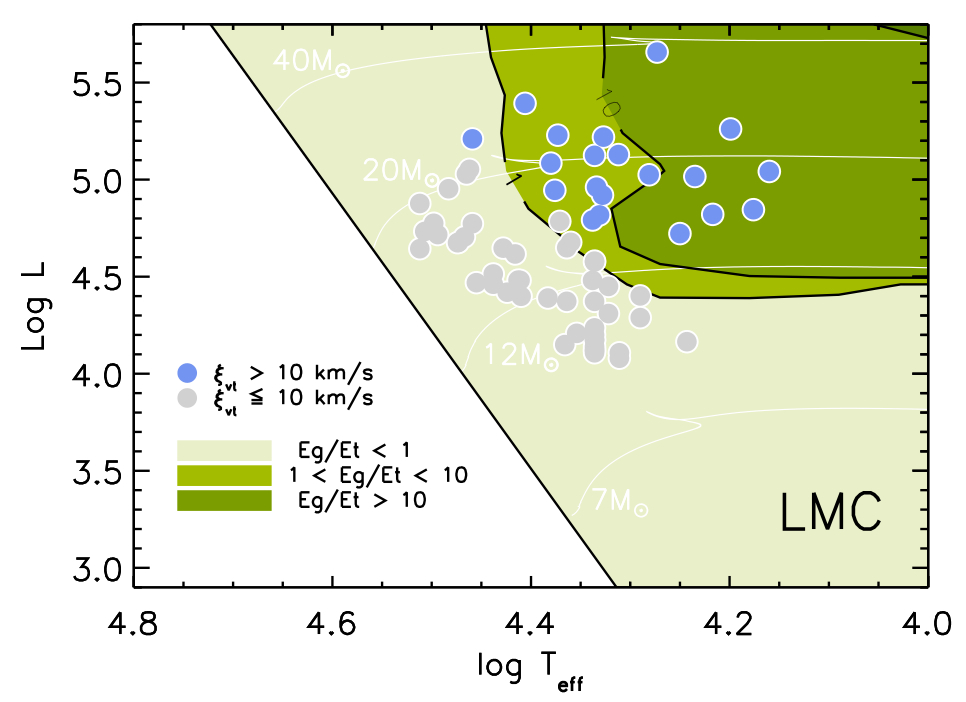
\includegraphics[width=0.7\columnwidth]{figures/figure_1/figure_1.jpg}
\caption{\subsection{Figures}
All figures should be submitted as separate files (with the figure legends at the end of the main article file). Please do not submit any figures that have been previously copyrighted unless you have express written permission from the copyright holder (usually the Publisher unless the publication is open access) to publish under the Creative Commons Attribution License.
For clinical photographs, please ensure you have appropriate written consent to publish them from the patient involved.

}
\end{center}
\end{figure}

\section*{Discussion}
The discussion should include the implications of the article results in view of prior work in this field.
For Data Articles, this section should not be included. 


\section*{Conclusions}
Please state what you think are the main conclusions that can be realistically drawn from the findings in the paper, taking care not to make claims that cannot be supported.

\section*{Consent}
The consent statement is required for articles involving patient data or information (e.g. personal genomics articles, case reports, clinical trials etc). You must ensure you have written informed consent from all the patients involved (or their legal guardian for a minor, or next of kin if the patient is deceased).

Please therefore add a line in your article under this heading stating 'Written informed consent for publication of their clinical details and/or clinical images was obtained from the patient/parent/guardian/ relative of the patient.'

\section*{Author contributions}
In order to give appropriate credit to each author of an article, the individual contributions of each author to the manuscript should be detailed in this section. We recommend using author initials and then stating briefly how they contributed.

\section*{Competing Interests}
All financial, personal, or professional competing interests for any of the authors that could be construed to unduly influence the content of the article must be disclosed and will be displayed alongside the article.
If you do not feel you have any relevant financial or non-financial competing interests to disclose, please include the line: 'No competing interests were disclosed' in this section. 

\section*{Grant Information}
Please state who funded the work discussed in this article, whether it is your employer, a grant funder etc. Please do not list funding that you have that is not relevant to this specific piece of research. For each funder, please state the funder{'}s name, the grant number where applicable, and the individual to whom the grant was assigned.

If your work was not funded by any grants, please include the line: {'}The author(s) declared that no grants were involved in supporting this work.{'}

\section*{Acknowledgements}
This section should acknowledge anyone who contributed to the research or the
article but who does not qualify as an author based on the criteria provided earlier
(e.g. someone or an organisation that provided writing assistance). Please state how
they contributed; authors should obtain permission to acknowledge from all those
mentioned in the Acknowledgements section.

Please do not list grant funding in this section (this should be included in the Grant information section - See above).

\section{References}
References can be listed in any standard referencing style that uses a {\bf numbering} system (i.e. not Harvard referencing style), and should be consistent between references within a given article. However, key points include:
\begin{itemize}
\item Journal abbreviations should follow the Index Medicus/MEDLINE abbreviation approach.
\end{itemize}
\begin{itemize}
\item Datasets should be cited in the reference section and should follow one of these examples.
\end{itemize}
\begin{itemize}
\item Only articles, datasets and abstracts that have been published or are in press, or are available through public e-print/preprint servers/data repositories, may be cited. Unpublished abstracts, papers that have been submitted but not yet accepted, and personal communications should instead be included in the text, and should be referred to as {'}personal communications{'} or {'}unpublished reports{'} and the researchers involved should be named. It is the responsibility of the authors to ensure they obtain permission to quote any personal communications from the cited individuals.
\end{itemize}
\begin{itemize}
\item Web links, URLs, and links to the authors{'} own websites should be included as hyperlinks within the authors' manuscript (e.g. 'Mouse Tumor Biology Database'), and not as references.
\end{itemize}
\begin{itemize}
\item References to trials on a clinical trial database should be as follows:
[Authors/name of group], [title of the trial], In: ClinicalTrials.gov [cited year month date], Available from [URL of the link from ClinicalTrials.gov] e.g. Kovacs Foundation, The Effect of Ozone Therapy for Lumbar Herniated Disc. In: ClinicalTrials.gov [cited 2012 Aug 30], Available from http://clinicaltrials.gov/ct2/show/NCT00566007
\end{itemize}


\section*{Figure Legends}
Please insert all figure legends at the end of your article. 

\textbf{\label{fig:fig1} Figure Title.} Each figure title should consist of no more than 15 words. Your figure legend should be succinct, while still explaining all symbols and abbreviations. 


\bibliography{bibliography/converted_to_latex.bib}

\end{document}

